% Template for theses recommended at Czech Technical University, Faculty of Information Technology
% inspired by lipics-v2019 documentclass
% Questions and help: <ondrej.guth@fit.cvut.cz>
% 2021: work in progress

\documentclass[a4paper,czech,unicode,twoside]{book}[2019/12/20]

%%%%%%%%%%%%%%%%%%%%%%%%%%%%%%%%%%
% FILL IN THIS INFORMATION
%%%%%%%%%%%%%%%%%%%%%%%%%%%%%%%%%%
\newcommand{\thesistitle}{Název příkladné závěrečné práce}
\newcommand{\thesistype}{Bakalářská práce}
\newcommand{\thesisauthor}{Jiří Nebozíz}
\newcommand{\supervisor}{doc.\,Ing.\,Damien Zlo,\,Ph.D.}
\newcommand{\department}{Katedra teoretické informatiky}
\newcommand{\yearofdefence}{2021}
%%%%%%%%%%%%%%%%%%%%%%%%%%%%%%%%%%
% END FILL IN
%%%%%%%%%%%%%%%%%%%%%%%%%%%%%%%%%%

%%%%%%%%%%%%%%%%%%%%%%%%%%%%%%%%%%
% TEMPLATE SETTINGS
% no need to modify anything within this section
%%%%%%%%%%%%%%%%%%%%%%%%%%%%%%%%%%
\title{\thesistitle}
\author{\thesisauthor}
\RequirePackage{babel}[2020/07/13] %localization
\RequirePackage{iftex}[2020/03/06]
\iftutex
    \RequirePackage{ellipsis}[2020/05/22] %ellipsis workaround for XeLaTeX
\else
    \RequirePackage[utf8]{inputenc}[2018/08/11] %this file encoding
    \RequirePackage{lmodern}[2009/10/30]
\fi
\RequirePackage[bottom=4cm,footskip=4em]{geometry}[2020/01/02] %page layout
\RequirePackage{setspace}[2011/12/19] %line spacing in title page
\RequirePackage{listings}[2020/03/24]
\RequirePackage{xcolor}[2016/05/11]
\RequirePackage{multicol}[2019/12/09]
\RequirePackage{titlesec}[2019/10/16]
\RequirePackage{mathtools}[2020/03/24]
\RequirePackage{amssymb}[2013/01/14]
\RequirePackage[pdfpagelayout=TwoPageRight]{hyperref}[2020-05-15] % optional package
\RequirePackage{pdfpages}[2020/01/28]
\RequirePackage{fancyhdr}[2019/01/31]
\RequirePackage[labelsep=space,singlelinecheck=false,font={up,small},labelfont={sf,bf}]{caption}[2020/05/30]
\RequirePackage{amsthm}[2020/05/29]
\RequirePackage{emptypage}[2010/05/30]

%%% modra
 \definecolor{decoration}{RGB}{0, 122, 195} %CTU blue
 \definecolor{heading}{RGB}{0, 122, 195}
 \definecolor{headbackgroundgray}{RGB}{199, 219, 241} %light blue
 \definecolor{backgroundgray}{RGB}{199, 219, 241} %CTU light blue
 \definecolor{headgray}{rgb}{0.50,0.50,0.51}
 \definecolor{enumgray}{RGB}{0, 122, 195} %CTU blue

\bibliographystyle{plainurl}% the mandatory bibstyle

\setcounter{secnumdepth}{4}% numbering sections; 4: subsubsection

% code listing settings
\renewcommand\lstlistingname{Výpis kódu}
\renewcommand\lstlistlistingname{Seznam výpisů kódu}
\lstset{basicstyle=\small\ttfamily,keywordstyle=\bfseries,%
        backgroundcolor=\color{backgroundgray},%
        frame=single,framerule=0pt,xleftmargin=\fboxsep,xrightmargin=\fboxsep}
% code listing setting end

% captions settings
\makeatletter
\@ifpackagelater{hyperref}{2009/12/09}
  {\captionsetup{compatibility=false}}%cf. http://groups.google.de/group/comp.text.tex/browse_thread/thread/db9310eb540fbbd8/42e30f3b7b3aa17a?lnk=raot
  {}
\makeatother
\DeclareCaptionLabelFormat{boxed}{%0.61,0.61,0.61
  \kern0.05em{\color{decoration}\rule{0.73em}{0.73em}}%
  \hspace*{0.67em}\bothIfFirst{#1}{~}#2}
\captionsetup{labelformat=boxed}
\captionsetup[table]{position=top}
% captions settings end

% lists settings
\setlength\leftmargini  \parindent
\setlength\leftmarginii {1.2em}
\setlength\leftmarginiii{1.2em}
\setlength\leftmarginiv {1.2em}
\setlength\leftmarginv  {1.2em}
\setlength\leftmarginvi {1.2em}
\renewcommand\labelenumi{%
  \textcolor{enumgray}{\headfont\bfseries\upshape\mathversion{bold}\theenumi.}}
\renewcommand\labelenumii{%
  \textcolor{enumgray}{\headfont\bfseries\upshape\mathversion{bold}\theenumii.}}
\renewcommand\labelenumiii{%
  \textcolor{enumgray}{\headfont\bfseries\upshape\mathversion{bold}\theenumiii.}}
\renewcommand\labelenumiv{%
  \textcolor{enumgray}{\headfont\bfseries\upshape\mathversion{bold}\theenumiv.}}
\makeatletter
\renewcommand\labelitemi{%
  \textcolor{enumgray}{\ifnum\@listdepth=\@ne
                                  \rule{0.67em}{0.33em}%
                                \else
                                  \rule{0.45em}{0.225em}%
                                \fi}}
\makeatother
\renewcommand\labelitemii{%
  \textcolor{enumgray}{\rule{0.45em}{0.225em}}}
\renewcommand\labelitemiii{%
  \textcolor{enumgray}{\headfont\bfseries\textasteriskcentered}}
\renewcommand\labelitemiv{%
  \textcolor{enumgray}{\headfont\bfseries\textperiodcentered}}
\renewcommand*\descriptionlabel[1]{%
  \hspace\labelsep\textcolor{enumgray}{\headfont\bfseries\mathversion{bold}#1}}
% lists settings end

\def\headfont{\rmfamily} %font for headings (chapter, section, etc.)

% frontmatter headings
\def\frontchapterfont{\Large \bfseries}
\def\frontsectionfont{\large\bfseries}
\def\frontsubsectionfont{\large}
\def\frontsubsubsectionfont{\bfseries}
% frontmatter headings end

% frontmatter pseudochapters: named part without printing actual chapter heading
\makeatletter
\newcommand{\frontchapternotprinted}[1]{%
  \begingroup
  \let\@makechapterhead\@gobble % make \@makechapterhead do nothing
  \let\cleardoublepage\clearpage
  \chapter{#1}
  \endgroup
}
\makeatother
% frontmatter pseudochapters end

% theorems, proofs, definitions, etc. end
\makeatletter
\thm@headfont{%
  \textcolor{decoration}{$\blacktriangleright$}\nobreakspace\headfont\bfseries}
\def\th@remark{%
  \thm@headfont{%
    \textcolor{decoration}{$\blacktriangleright$}\nobreakspace\headfont}%
  \normalfont % body font
  \thm@preskip\topsep \divide\thm@preskip\tw@
  \thm@postskip\thm@preskip
}
\def\@endtheorem{\endtrivlist}%\@endpefalse
\renewcommand\qedsymbol{\textcolor{decoration}{\ensuremath{\blacktriangleleft}}}
\renewenvironment{proof}[1][\proofname]{\par
  \pushQED{\qed}%
  \normalfont \topsep6\p@\@plus6\p@\relax
  \trivlist
  \item[\hskip\labelsep
        \color{black}\headfont\bfseries
    #1\@addpunct{.}]\ignorespaces
}{%
  \popQED\endtrivlist%\@endpefalse
}
\makeatother
\theoremstyle{plain}
\newtheorem{theorem}{Věta}
\newtheorem{lemma}[theorem]{Pomocné tvrzení}
\newtheorem{corollary}[theorem]{Důsledek}
\newtheorem{proposition}[theorem]{Návrh}
\newtheorem{definition}[theorem]{Definice}
\theoremstyle{definition}
\newtheorem{example}[theorem]{Příklad}
\theoremstyle{remark}
\newtheorem{note}[theorem]{Poznámka}
\newtheorem*{note*}{Poznámka}
\newtheorem{remark}[theorem]{Pozorování}
\newtheorem*{remark*}{Pozorování}
\numberwithin{theorem}{chapter}
% theorems, proofs, definitions, etc. end

% table of contents colored chapters
\makeatletter
\let\stdl@chapter\l@chapter
\renewcommand*{\l@chapter}[2]{%
  \stdl@chapter{\textcolor{heading}{#1}}{\textcolor{heading}{#2}}}
\makeatother
% table of contents colored chapters end

% headers and footers
\makeatletter
\def\ps@plain{%chapter beginning
    \let\@evenhead\@empty%
    \let\@oddhead\@empty%
    \def\@evenfoot{\bfseries\color{headgray}\hfill\thepage\hfill}%
    \def\@oddfoot{\bfseries\color{headgray}\hfill\thepage\hfill}}
\makeatother
\renewcommand{\chaptermark}[1]{\markboth{#1}{}}
\renewcommand{\sectionmark}[1]{\markright{#1}}
\pagestyle{fancy}
\fancyhf{}
\fancyhead[LE]{\leavevmode\smash{\llap{\color{headgray} \bfseries \thepage \hspace*{4em}}}}
\fancyhead[RE]{\color{headgray}\bfseries\nouppercase{\leftmark}}
\fancyhead[RO]{\leavevmode\smash{\rlap{\hspace*{4em}\color{headgray}\bfseries\thepage}}}
\fancyhead[LO]{\color{headgray}\bfseries\nouppercase{\rightmark}}
\renewcommand{\headrulewidth}{0pt}
% headers and footers end

% title page
\renewcommand{\maketitle}{\begin{titlepage}%
\newgeometry{left=67mm,top=80mm,right=40mm}%\thispagestyle{empty}%
\noindent{\large\headfont\noindent\thesistype}
\vskip 3mm
\noindent{\noindent\huge\headfont\bfseries\color{black}\begin{flushleft}\begin{onehalfspace}\MakeUppercase{\thesistitle}\end{onehalfspace}\end{flushleft}}
\vskip 35mm
\noindent{\large \headfont \bfseries \thesisauthor}

\vfill

\noindent{\headfont Fakulta informačních technologií ČVUT v Praze\\
\department\\
Vedoucí: \supervisor\\
\today}\end{titlepage}
\restoregeometry
}
%title page end

\newenvironment{abstrakt}{%
  \vspace*{18mm}
  \noindent
  {{\frontchapterfont\begin{flushleft}{\color{heading}Abstrakt}\end{flushleft}}}%
  \bigskip
  \noindent\ignorespaces}

\newenvironment{abstract}{%
  \vskip\bigskipamount
  \noindent
  {{\frontchapterfont\begin{flushleft}{\color{heading}Abstract}\end{flushleft}}}%
  \bigskip
  \noindent\ignorespaces}
  
\newenvironment{prohlaseni}{
  {{\frontchapterfont\begin{flushright}{\color{heading}Prohlášení}\end{flushright}}}%
  \bigskip
  \noindent\ignorespaces}

%%%%%%%%%%%%%%%%%%%%%%%%%%%%%%%%%%
% TEMPLATE SETTINGS END
%%%%%%%%%%%%%%%%%%%%%%%%%%%%%%%%%%


%%%%%%%%%%%%%%%%%%%%%%
% DEMO CONTENTS SETTINGS
% You may choose to modify this part.
%%%%%%%%%%%%%%%%%%%%%%
\usepackage{dirtree}
\usepackage{lipsum,tikz}
%%%%%%%%%%%%%%%%%%%%%%
% DEMO CONTENTS SETTINGS END
%%%%%%%%%%%%%%%%%%%%%%

\begin{document}
\frontmatter
%%%%%%%%%%%%%%
% FRONTMATTER SETTINGS
% no need to modify this part
%%%%%%%%%%%%%%
\titleformat
{\chapter} % command
% [display] % shape
{} % format
{} % label
{} % sep
{\color{heading}\frontchapterfont \raggedleft} % before-code
[\vskip -2em] % after-code

\titleformat
{\section}
{\frontsectionfont\color{heading}}
{}
{}
{}
  
% \titleformat{\subsection}
%   {\frontsubsectionfont\color{heading}}{{{\color{black}\thesubsection}}}{1em}{}[\vskip -1em]
  
% \titleformat{\subsubsection}
%   {\frontsubsubsectionfont\color{heading}}{{{\color{black}\thesubsubsection}}}{1em}{}[\vskip -1em]

\makeatletter
\@openrightfalse
\makeatother
%%%%%%%%%%%%%%
% FRONTMATTER SETTINGS END
%%%%%%%%%%%%%%


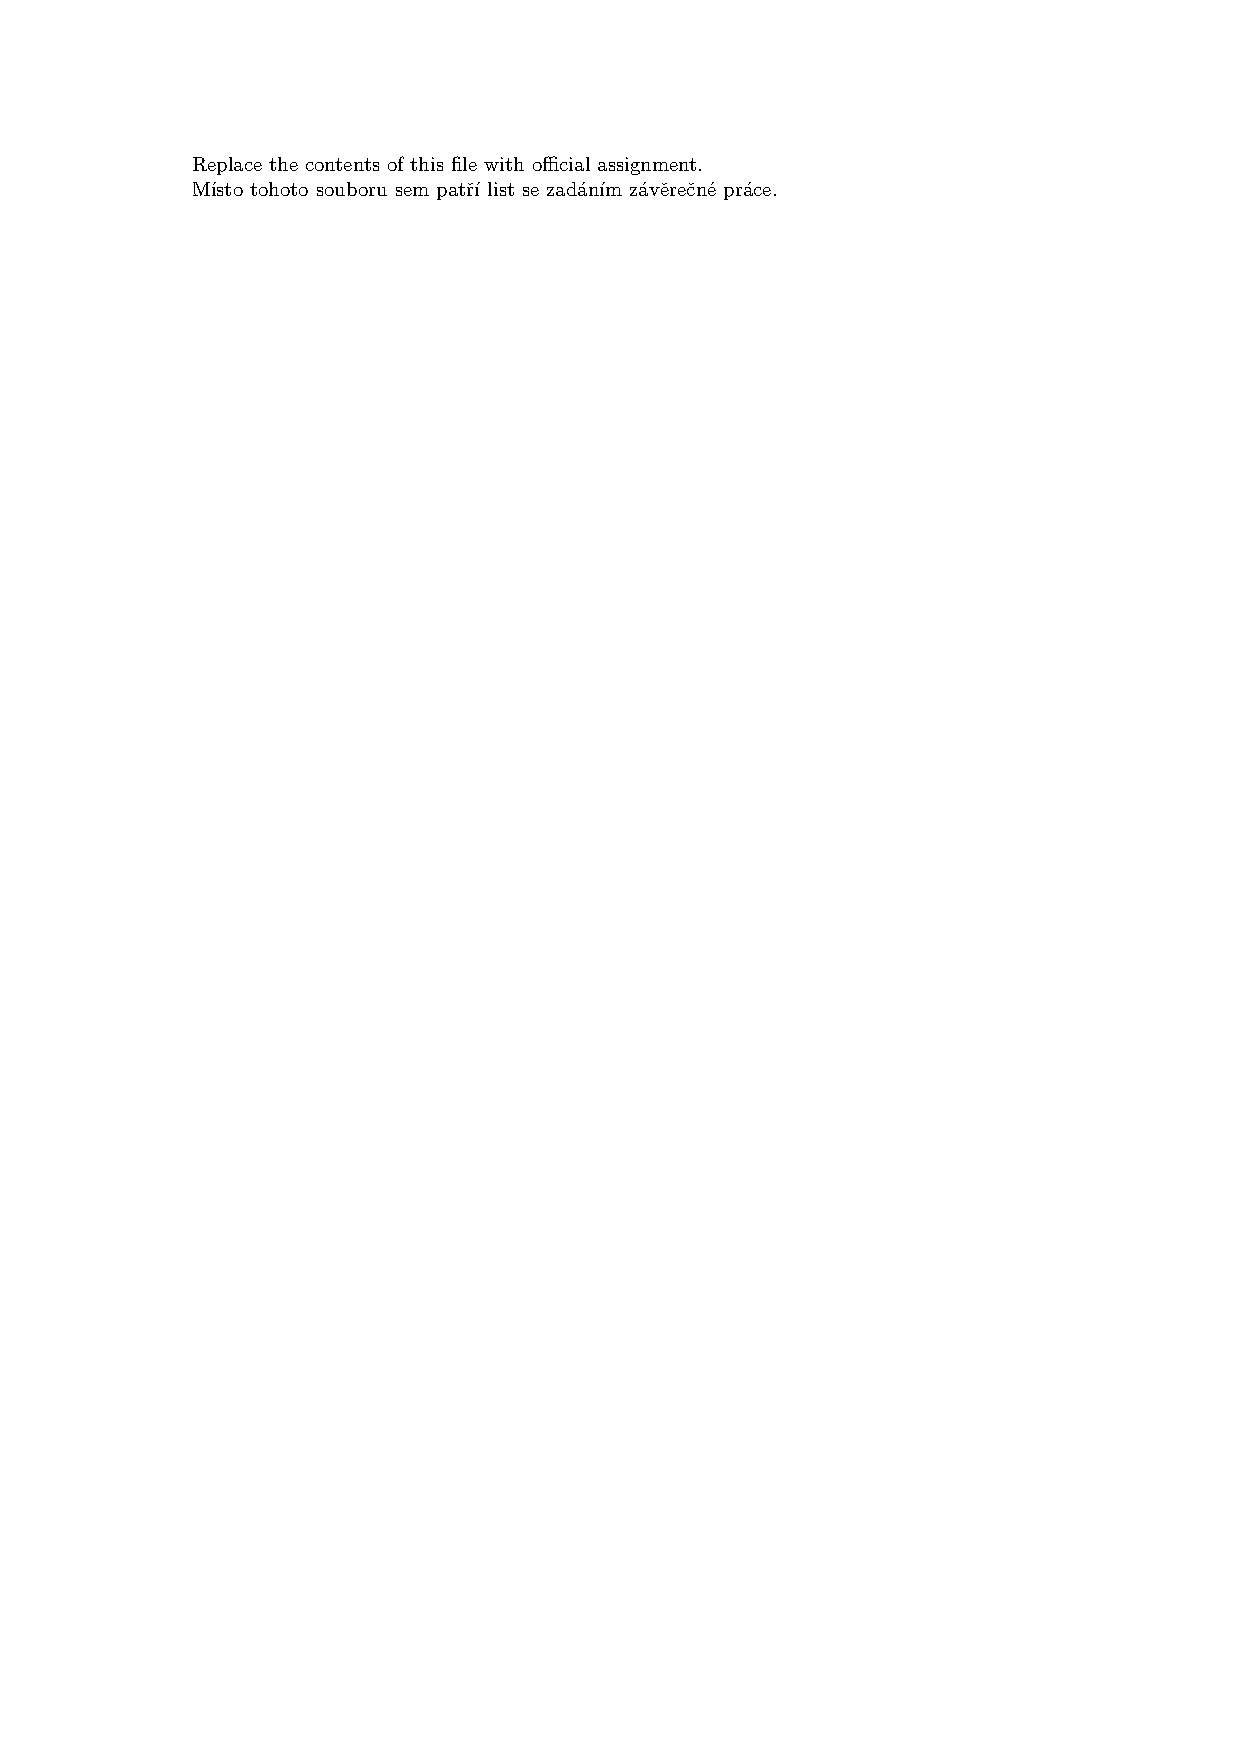
\includepdf{assignment-include.pdf}

\thispagestyle{empty}
\cleardoublepage

\maketitle
% \clearpage

%%%%%%%%%%%%%%%%%%%%%%%%%%%%%%
% PREPRINT
% no need to modify
%%%%%%%%%%%%%%%%%%%%%%%%%%%%%%

	\clearpage
	\thispagestyle{empty}
	

		~
	\vfill
	
	{\small
			\noindent České vysoké učení technické v Praze \\
		\noindent Fakulta informačních technologií \\
	\noindent \textcopyright{} \yearofdefence{} \thesisauthor. Všechna práva vyhrazena.\\
		\noindent \textit{Tato práce vznikla jako školní dílo na Českém vysokém učení technickém v Praze, Fakultě informačních technologií. Práce je chráněna právními předpisy a mezinárodními úmluvami o právu autorském a právech souvisejících s právem autorským. K jejímu užití, s výjimkou bez uplatněných zákonných licencí nad rámec oprávnění uvedených v Prohlášení, je nezbytný souhlas autora.}
	
	\vspace{1em}
	
	\noindent Odkaz na tuto práci: \thesisauthor. \textit{\thesistitle}. \thesistype. České vysoké učení technické v Praze, Fakulta informačních technologií, \yearofdefence.
}
%%%%%%%%%%%%%%%%%%%%%%%%%%%%%%
% PREPRINT END
%%%%%%%%%%%%%%%%%%%%%%%%%%%%%%

\tableofcontents
\listoffigures
\begingroup
\let\clearpage\relax
\listoftables
\lstlistoflistings
\endgroup

%%%%%%%%%%%%%%%%%%%
% ACKNOWLEDGMENT
% FILL IN / MODIFY
%%%%%%%%%%%%%%%%%%%
\frontchapternotprinted{Poděkování}
~
\vfill
\hskip 0cm \begin{minipage}{0.7\textwidth}
\textit{Chtěl bych poděkovat především sit amet, consectetuer adipiscing elit. Curabitur sagittis hendrerit ante. Class aptent taciti sociosqu ad litora torquent per conubia nostra, per inceptos hymenaeos. Cras pede libero, dapibus nec, pretium sit amet, tempor quis. Sed vel lectus. Donec odio tempus molestie, porttitor ut, iaculis quis, sem. Suspendisse sagittis ultrices augue.}
\end{minipage}

\vfill

\vfill
%%%%%%%%%%%%%%%%%%%
% ACKNOWLEDGMENT END
%%%%%%%%%%%%%%%%%%%



%%%%%%%%%%%%%%%%%%%
% ACKNOWLEDGMENT
% FILL IN / MODIFY
%%%%%%%%%%%%%%%%%%%
\frontchapternotprinted{Prohlášení}
~
\vfill
% INSTRUCTIONS
% ENG: choose one of approved texts of the declaration. DO NOT CREATE YOUR OWN. Find the approved texts at https://courses.fit.cvut.cz/SFE/download/index.html#_documents (document Declaration for FT in English)
% CZE/SLO: Vyberte jedno z fakultou schvalenych prohlaseni. NEVKLADEJTE VLASTNI TEXT. Schvalena prohlaseni najdete zde: https://courses.fit.cvut.cz/SZZ/dokumenty/index.html#_dokumenty (prohlášení do ZP)
\begin{prohlaseni}
Lorem ipsum dolor sit amet, consectetuer adipiscing elit. Curabitur sagittis hendrerit ante. Class aptent taciti sociosqu ad litora torquent per conubia nostra, per inceptos hymenaeos. Cras pede libero, dapibus nec, pretium sit amet, tempor quis. Sed vel lectus. Donec odio tempus molestie, porttitor ut, iaculis quis, sem. Suspendisse sagittis ultrices augue. Donec ipsum massa, ullamcorper in, auctor et, scelerisque sed, est. In sem justo, commodo ut, suscipit at, pharetra vitae, orci. Pellentesque pretium lectus id turpis.

Lorem ipsum dolor sit amet, consectetuer adipiscing elit. Curabitur sagittis hendrerit ante. Class aptent taciti sociosqu ad litora torquent per conubia nostra, per inceptos hymenaeos. Cras pede libero, dapibus nec, pretium sit amet, tempor quis. Sed vel lectus. Donec odio tempus molestie, porttitor ut, iaculis quis, sem. Suspendisse sagittis ultrices augue. Donec ipsum massa, ullamcorper in, auctor et, scelerisque sed, est. In sem justo, commodo ut, suscipit at, pharetra vitae, orci. Pellentesque pretium lectus id turpis.
\vskip 1cm
\noindent
V Praze dne 10.\;května 2020 \hspace{.3\textwidth} \dotfill
\end{prohlaseni}
%%%%%%%%%%%%%%%%%%%
% DECLARATION END
%%%%%%%%%%%%%%%%%%%



%%%%%%%%%%%%%%%%%%%
% ABSTRACT
% FILL IN / MODIFY
%%%%%%%%%%%%%%%%%%%
\frontchapternotprinted{Abstrakt}
\begin{abstrakt}% Enter abstract in CZECH.
\lipsum[1]
\end{abstrakt}

\vskip 0.5cm

{\noindent\color{heading}\bfseries\headfont Klíčová slova\hspace{1em}}{lorem, ipsum dolor, sit amet}

\vskip 1cm

\begin{abstract}% Enter abstract in ENGLISH.
\lipsum[2]  
\end{abstract}

\vskip 0.5cm

{\noindent\color{heading}\bfseries\headfont Keywords\hspace{1em}}{lorem, ipsum dolor, sit amet}
%%%%%%%%%%%%%%%%%%%
% ABSTRACT END
%%%%%%%%%%%%%%%%%%%

%%%%%%%%%%%%%%%%%%%
% SUMMARY
% FILL IN / MODIFY
% OR REMOVE ENTIRELY (upon agreement with your supervisor)
% (apropriate to remove in most theses)
%%%%%%%%%%%%%%%%%%%
\chapter{Shrnutí}
\setlength{\columnsep}{1cm}
\begin{multicols}{2}
{\small

\section*{Motivace}

\lipsum[1][1-8]

\section*{Cíl práce}

\lipsum[2][1-6]

\section*{Postup}

\lipsum[3]

\section*{Výsledky práce}

\lipsum[2]

\section*{Závěr}

\lipsum[1][1-8] Lorem lorem lorem.
}
\end{multicols}
%%%%%%%%%%%%%%%%%%%
% SUMMARY END
%%%%%%%%%%%%%%%%%%%

%%%%%%%%%%%%%%%%%%%
% ABBREVIATIONS
% FILL IN / MODIFY
% OR REMOVE ENTIRELY
%%%%%%%%%%%%%%%%%%%
\chapter{Seznam zkratek}
	
\begin{tabular}{rl}
DFA & Deterministic Finite Automaton\\
FA & Finite Automaton\\
LPS & Labelled Prüfer Sequence\\
NFA & Nondeterministic Finite Automaton\\
NPS & Numberef Prüfer Sequence\\
TPA & Tree Paths Automaton\\
TSPA & Tree String Paths Subsequences Automaton\\
XML & Extensible Markup Language\\
XPath & XML Path Language\\
XSLT & eXtensible Stylesheet Language Transformations\\
W3C & World Wide Web Consortium
\end{tabular}
%%%%%%%%%%%%%%%%%%%
% ABBREVIATIONS END
%%%%%%%%%%%%%%%%%%%

\mainmatter

%%%%%%%%%%%%%%%%%%%%
% MAINMATTER SETTINGS
% no need to modify this part
%%%%%%%%%%%%%%%%%%%%
\makeatletter
\@openrighttrue
\makeatother

\titleformat
{\chapter} % command
[display] % shape
{\headfont \LARGE \bfseries \raggedleft} % format
{ \textcolor{headbackgroundgray}{{\titlerule*[1pc]{\rule{0.25em}{0.25em}}}} \hspace{0.5ex} \color{black} Kapitola \thechapter } % label
{-0.3cm} % sep
{\color{heading} \Huge \vskip 0.5cm} % before-code
[\vskip 1cm] % after-code

%vzhled nadpisů sekcí
\titleformat{\section}
  {\headfont\Large\bfseries\color{heading}}{\colorbox{headbackgroundgray}{{\color{black}\thesection}}}{1em}{}%[\vskip -1em]
  
\titleformat{\subsection}
  {\headfont\Large\bfseries\color{heading}}{{{\color{black}\thesubsection}}}{1em}{}%[\vskip -1em]
  
\titleformat{\subsubsection}
  {\headfont\large\bfseries\color{heading}}{{{\color{black}\thesubsubsection}}}{1em}{}%[\vskip -1em]

%%%%%%%%%%%%%%%%%%%%
% MAINMATTER SETTINGS END
%%%%%%%%%%%%%%%%%%%%

%%%%%%%%%%%%%%%%%%%
% THE THESIS
% MODIFY ANYTHING BELOW THIS LINE
%%%%%%%%%%%%%%%%%%%
% Do not forget to include Introduction
%---------------------------------------------------------------
% \chapter{Introduction}
% uncomment the following line to create an unnumbered chapter
\chapter*{Introduction}\addcontentsline{toc}{chapter}{Introduction}\markboth{Introduction}{Introduction}
%---------------------------------------------------------------
\setcounter{page}{1}

% The following environment can be used as a mini-introduction for a chapter. Use that any way it pleases you (or comment it out). It can contain, for instance, a summary of the chapter. Or, there can be a quotation.
\begin{chapterabstract}
	\lipsum[1]
\end{chapterabstract}

\lipsum[2][1-4]{} [1]

\lipsum[4]

%---------------------------------------------------------------
\section{Ut enim ad minim veniam}
%---------------------------------------------------------------

\lipsum[6-7]

\begin{figure}
\centering
%\includegraphics[scale=0.4]{pic/index}
\resizebox{\textwidth}{!}{
\begin{tikzpicture}[level/.style={sibling distance=60mm/#1}]
\node [circle,draw] (z){$n$}
  child {node [circle,draw] (a) {$\frac{n}{2}$}
    child {node [circle,draw] (b) {$\frac{n}{2^2}$}
      child {node {$\vdots$}
        child {node [circle,draw] (d) {$\frac{n}{2^k}$}}
        child {node [circle,draw] (e) {$\frac{n}{2^k}$}}
      } 
      child {node {$\vdots$}}
    }
    child {node [circle,draw] (g) {$\frac{n}{2^2}$}
      child {node {$\vdots$}}
      child {node {$\vdots$}}
    }
  }
  child {node [circle,draw] (j) {$\frac{n}{2}$}
    child {node [circle,draw] (k) {$\frac{n}{2^2}$}
      child {node {$\vdots$}}
      child {node {$\vdots$}}
    }
  child {node [circle,draw] (l) {$\frac{n}{2^2}$}
    child {node {$\vdots$}}
    child {node (c){$\vdots$}
      child {node [circle,draw] (o) {$\frac{n}{2^k}$}}
      child {node [circle,draw] (p) {$\frac{n}{2^k}$}
          child [grow=right] {node (q) {$ = O_{k = \lg n}(n)$} edge from parent[draw=none]
            child [grow=up] {node (r) {$\vdots$} edge from parent[draw=none]
              child [grow=up] {node (s) {$O_2(n)$} edge from parent[draw=none]
                child [grow=up] {node (t) {$O_1(n)$} edge from parent[draw=none]
                  child [grow=up] {node (u) {$O_0(n)$} edge from parent[draw=none]}
                }
              }
            }
            child [grow=down] {node (v) {$O(n \cdot \lg n)$}edge from parent[draw=none]}
        }
      }
    }
  }
};
\path (a) -- (j) node [midway] {+};
\path (b) -- (g) node [midway] {+};
\path (k) -- (l) node [midway] {+};
\path (k) -- (g) node [midway] {+};
\path (d) -- (e) node [midway] {+};
\path (o) -- (p) node [midway] {+};
\path (o) -- (e) node (x) [midway] {$\cdots$}
  child [grow=down] {
    node (y) {$O\left(\displaystyle\sum_{i = 0}^k 2^i \cdot \frac{n}{2^i}\right)$}
    edge from parent[draw=none]
  };
\path (q) -- (r) node [midway] {+};
\path (s) -- (r) node [midway] {+};
\path (s) -- (t) node [midway] {+};
\path (s) -- (l) node [midway] {=};
\path (t) -- (u) node [midway] {+};
\path (z) -- (u) node [midway] {=};
\path (j) -- (t) node [midway] {=};
\path (y) -- (x) node [midway] {$\Downarrow$};
\path (v) -- (y)
  node (w) [midway] {$O\left(\displaystyle\sum_{i = 0}^k n\right) = O(k \cdot n)$};
\path (q) -- (v) node [midway] {=};
\path (e) -- (x) node [midway] {+};
\path (o) -- (x) node [midway] {+};
\path (y) -- (w) node [midway] {$=$};
\path (v) -- (w) node [midway] {$\Leftrightarrow$};
\path (r) -- (c) node [midway] {$\cdots$};
\end{tikzpicture}}
\caption{~Lorem ipsum dolor sit amet}\label{img:index}
\end{figure}

%---------------------------------------------------------------
\section{Ut enim ad minim veniam}
%---------------------------------------------------------------

\lipsum[2-4]

%---------------------------------------------------------------
\subsection{Ut enim ad minim veniam}
%---------------------------------------------------------------

Curabitur ligula sapien, pulvinar a vestibulum quis, facilisis vel sapien. Duis condimentum augue id magna semper rutrum. Aliquam ornare wisi eu metus. Fusce aliquam vestibulum ipsum. Vivamus ac leo pretium faucibus\ref{img:index}.

\begin{itemize}
    \item Ut enim ad minim veniam, quis nostrud
    \item Ut enim ad minim 
    \item Ut enim ad minim veniam, quis 
    \begin{itemize}
        \item Ut enim ad
        \item Ut enim ad
        \begin{itemize}
            \item Ut enim 
            \item Ut enim 
            \begin{itemize}
            \item Ut enim 
            \item Ut enim 
        \end{itemize}
        \end{itemize}
    \end{itemize}
\end{itemize}

\section{Class aptent taciti}

\lipsum[2]

\subsection{Class aptent taciti}

\lipsum[6-7]

\begin{enumerate}
    \item Ut enim ad minim veniam, quis nostrud
    \item Ut enim ad minim 
    \item Ut enim ad minim veniam, quis 
    \begin{enumerate}
        \item Ut enim ad
        \item Ut enim ad
        \begin{enumerate}
            \item Ut enim 
            \item Ut enim 
            \begin{enumerate}
            \item Ut enim 
            \item Ut enim 
        \end{enumerate}
        \end{enumerate}
    \end{enumerate}
\end{enumerate}


%---------------------------------------------------------------
\section{Ut enim ad minim veniam, quis nostrud}
%---------------------------------------------------------------

Ut enim ad minim veniam, quis nostrud exercitation ullamco laboris nisi ut aliquip ex ea commodo consequat. Nulla non arcu lacinia neque faucibus fringilla. Vestibulum erat nulla, ullamcorper nec, rutrum non, nonummy ac, erat. Aliquam erat volutpat. Proin pede metus, vulputate nec, fermentum fringilla, vehicula vitae, justo.\footnote{Ut enim ad minim veniam, quis nostrud exercitation.} Etiam dictum tincidunt diam. In laoreet, magna id viverra tincidunt, sem odio bibendum justo, vel imperdiet sapien wisi sed libero. Nulla est. Maecenas fermentum, sem in pharetra pellentesque, velit turpis volutpat ante, in pharetra metus odio a lectus. Duis aute irure dolor in reprehenderit in voluptate velit esse cillum dolore eu fugiat nulla pariatur. 

\begin{lstlisting}[caption={~Zbytečný kód},label=list:8-6,captionpos=t,float,abovecaptionskip=-\medskipamount,belowcaptionskip=\medskipamount,language=C]
    #include<stdio.h>
    #include<iostream>
    // A comment
    int main(void)
    {
        printf("Hello World\n");
        return 0;
    }
\end{lstlisting}

%%%%%%%%%%%%%%%%%%%%%%%%%%%%%%%%%
% alternative using package minted for source highlighting
% package minted requires execution with `-shell-escape'
% e.g., `xelatex -shell-escape ctufit-thesis.tex'
% \begin{listing}
% \caption{Zbytečný kód}\label{list:8-6}
% \begin{minted}{C}
%     #include<stdio.h>
%     #include<iostream>
%     // A comment
%     int main(void)
%     {
%         printf("Hello World\n");
%         return 0;
%     }
% \end{minted}
% \end{listing}
% %%%%%%%%%%%%%%%%%%%%%%%%%%%%%%%%%
Nullam feugiat, turpis at pulvinar vulputate, erat libero tristique tellus, nec bibendum odio risus sit amet ante. Aenean id metus id velit ullamcorper pulvinar. Fusce wisi. Integer lacinia. Aliquam id dolor. Pellentesque pretium lectus id turpis. Suspendisse sagittis ultrices augue. In laoreet, magna id viverra tincidunt, sem odio bibendum justo, vel imperdiet sapien wisi sed libero. Sed ac dolor sit amet purus malesuada congue. \cite{Crochemore2002}

Class aptent taciti sociosqu ad litora torquent per conubia nostra, per inceptos hymenaeos. Fusce suscipit libero eget elit. Etiam dui sem, fermentum vitae, sagittis id, malesuada in, quam. Aliquam id dolor. Curabitur bibendum justo non orci. Duis viverra diam non justo. Curabitur ligula sapien, pulvinar a vestibulum quis, facilisis vel sapien. Duis condimentum augue id magna semper rutrum. Aliquam ornare wisi eu metus. Fusce aliquam vestibulum ipsum. Vivamus ac leo pretium faucibus. \cite{Motwani2014}

%---------------------------------------------------------------
\subsection{Ut enim ad minim veniam, quis nostrud}
%---------------------------------------------------------------

Ut enim ad minim veniam, quis nostrud exercitation ullamco laboris nisi ut aliquip ex ea commodo consequat. Nulla non arcu lacinia neque faucibus fringilla. Vestibulum erat nulla, ullamcorper nec, rutrum non, nonummy ac, erat. Aliquam erat volutpat. Proin pede metus, vulputate nec, fermentum fringilla, vehicula vitae, justo. Etiam dictum tincidunt diam. In laoreet, magna id viverra tincidunt, sem odio bibendum justo. \cite{Sestakova2018} 

\begin{table}\centering
\caption[Příklad tabulky]{~Zadávání matematiky}\label{tab:matematika}
\begin{tabular}{l|l|c|c}
	Typ		& Prostředí		& \LaTeX{}ovská zkratka	& \TeX{}ovská zkratka	\tabularnewline \hline 
 	Text		& \verb|math|		& \verb|\(...\)|	& \verb|$...$|	\tabularnewline \hline
 	Displayed	& \verb|displaymath|	& \verb|\[...\]|	& \verb|$$...$$|	\tabularnewline 
\end{tabular}
\end{table}


Nulla est. Maecenas fermentum, sem in pharetra pellentesque, velit turpis volutpat ante, in pharetra metus odio a lectus. Duis aute irure dolor in reprehenderit in voluptate velit esse cillum dolore eu fugiat nulla pariatur. Nullam feugiat, turpis at pulvinar vulputate, erat libero tristique tellus, nec bibendum odio risus sit amet ante. Aenean id metus id velit ullamcorper pulvinar. 

\subsubsection{Class aptent taciti}

\begin{definition}[Optional label]
Class aptent taciti sociosqu ad litora torquent per conubia nostra, per inceptos hymenaeos. Fusce suscipit libero eget elit. Etiam dui sem, fermentum vitae, sagittis id, malesuada in, quam. Aliquam id dolor. Curabitur bibendum justo non orci.
\end{definition}

\begin{example}
Class aptent taciti sociosqu ad litora torquent per conubia nostra, per inceptos hymenaeos. Fusce suscipit libero eget elit. Etiam dui sem, fermentum vitae, sagittis id, malesuada in, quam. Aliquam id dolor. Curabitur bibendum justo non orci.
\end{example}

\paragraph{Nadpis 5. úrovně}

\begin{theorem}
Class aptent taciti sociosqu ad litora torquent per conubia nostra, per inceptos hymenaeos. Fusce suscipit libero eget elit. Etiam dui sem, fermentum vitae, sagittis id, malesuada in, quam. Aliquam id dolor. Curabitur bibendum justo non orci.
\end{theorem}

\begin{proof}
Fusce suscipit libero eget elit. Etiam dui sem, fermentum vitae, sagittis id, malesuada in, quam. Aliquam id dolor. Curabitur bibendum justo non orci.
\end{proof}

\paragraph{Level 5 heading}

\begin{corollary}
Fusce suscipit libero eget elit. Etiam dui sem, fermentum vitae, sagittis id, malesuada in, quam. Aliquam id dolor. Curabitur bibendum justo non orci.
\end{corollary}

\begin{proposition}
Fusce suscipit libero eget elit. Etiam dui sem, fermentum vitae, sagittis id, malesuada in, quam. Aliquam id dolor. Curabitur bibendum justo non orci.
\end{proposition}

\begin{note}
Fusce suscipit libero eget elit. Etiam dui sem, fermentum vitae, sagittis id, malesuada in, quam. Aliquam id dolor. Curabitur bibendum justo non orci.
\end{note}

\begin{remark}
Fusce suscipit libero eget elit. Etiam dui sem, fermentum vitae, sagittis id, malesuada in, quam. Aliquam id dolor. Curabitur bibendum justo non orci.
\end{remark}

\begin{lemma}
Class aptent taciti sociosqu ad litora torquent per conubia nostra, per inceptos hymenaeos. Fusce suscipit libero eget elit. Etiam dui sem, fermentum vitae, sagittis id, malesuada in, quam. Aliquam id dolor. Curabitur bibendum justo non orci.
\end{lemma}

\lipsum[1-2]

% \subsection{Class aptent taciti sociosqu}
% 
% \lipsum[4-5]

%---------------------------------------------------------------
\chapter{Lorem ipsum}
%---------------------------------------------------------------

\begin{chapterabstract}
	Lorem ipsum dolor sit amet, consectetuer adipiscing elit. Curabitur sagittis hendrerit ante. Class aptent taciti sociosqu ad litora torquent per conubia nostra, per inceptos hymenaeos. Cras pede libero, dapibus nec, pretium sit amet, tempor quis. Sed vel lectus. Donec odio tempus molestie, porttitor ut, iaculis quis, sem. Cras pede libero, dapibus nec, pretium sit amet, tempor quis. Sed vel lectus. 
\end{chapterabstract}

Lorem ipsum dolor sit amet, consectetuer adipiscing elit. Curabitur sagittis hendrerit ante. Class aptent taciti sociosqu ad litora torquent per conubia nostra, per inceptos hymenaeos. Cras pede libero, dapibus nec, pretium sit amet, tempor quis. Sed vel lectus. Donec odio tempus molestie, porttitor ut, iaculis quis, sem. Suspendisse sagittis ultrices augue. Donec ipsum massa, ullamcorper in, auctor et, scelerisque sed, est. In sem justo, commodo ut, suscipit at, pharetra vitae, orci. Pellentesque pretium lectus id turpis. \cite{Kopka2004}

\section{Donec odio tempus molestie}

\lipsum[2] \cite{def:1, def:2}

\subsection{Class aptent taciti}

\lipsum[2-3]

\begin{description}
\item[Kapitola 1] Lorem ipsum dolor sit amet, consectetuer adipiscing elit. Curabitur sagittis hendrerit ante. Class aptent taciti sociosqu ad litora torquent per conubia nostra, per inceptos hymenaeos. Cras pede libero, dapibus nec, pretium sit amet, tempor quis.

\item[Kapitola 2] Lorem ipsum dolor sit amet, consectetuer adipiscing elit. Curabitur sagittis hendrerit ante. Class aptent taciti sociosqu ad litora torquent per conubia nostra, per inceptos hymenaeos. Cras pede libero, dapibus nec, pretium sit amet, tempor quis.

\item[Kapitola 3] Lorem ipsum dolor sit amet, consectetuer adipiscing elit. Curabitur sagittis hendrerit ante. Class aptent taciti sociosqu ad litora torquent per conubia nostra, per inceptos hymenaeos. Cras pede libero, dapibus nec, pretium sit amet, tempor quis.

\item[Kapitola 4] Lorem ipsum dolor sit amet, consectetuer adipiscing elit. Curabitur sagittis hendrerit ante. Class aptent taciti sociosqu ad litora torquent per conubia nostra, per inceptos hymenaeos. Cras pede libero, dapibus nec, pretium sit amet, tempor quis.
\end{description}

\lipsum[2]

\section{Lorem ipsum dolor sit amet}

\lipsum[3-5]


\appendix

%%%%%%%%%%%%%%%%%%%%
% APPENDIX SETTINGS
% no need to modify this part
%%%%%%%%%%%%%%%%%%%%
\titleformat
{\chapter} % command
[display] % shape
{\headfont \LARGE \bfseries \raggedleft} % format
{ \textcolor{headbackgroundgray}{{\titlerule*[1pc]{\rule{0.25em}{0.25em}}}} \hspace{0.5ex} \color{black} Příloha \thechapter } % label
{-0.3cm} % sep
{\color{heading} \Huge \vskip 0.5cm} % before-code
[\vskip 1cm] % after-code

%%%%%%%%%%%%%%%%%%%%
% MAINMATTER SETTINGS END
%%%%%%%%%%%%%%%%%%%%


\chapter{Nějaká příloha}


Sem přijde to, co nepatří do hlavní části.


\backmatter

\bibliography{bib-database}

\chapter{Obsah příloh}
% Contents of the attachment

	\dirtree{%
		.1 /.
		.2 readme.txt\DTcomment{stručný popis obsahu média}.
		.2 exe\DTcomment{adresář se spustitelnou formou implementace}.
		.2 src.
		.3 impl\DTcomment{zdrojové kódy implementace}.
		.3 thesis\DTcomment{zdrojová forma práce ve formátu \LaTeX{}}.
		.2 text\DTcomment{text práce}.
		.3 thesis.pdf\DTcomment{text práce ve formátu PDF}.
	}



\end{document}
